% Данный файл распространяется под лицензией CC BY 4.0. Текст лицензии размещён на https://creativecommons.org/licenses/by/4.0/
% (c) Кафедра системного программирования, 2025

\documentclass[a4paper]{article}

\usepackage[a4paper, top=8mm, bottom=8mm, left=8mm, right=8mm]{geometry}
\usepackage{polyglossia}
\setdefaultlanguage[babelshorthands=true]{russian}
\setotherlanguage{english}
\usepackage{fontspec}
\setmainfont{Times New Roman}
\newfontfamily{\russianfonttt}[Scale=0.7]{Courier New}
\usepackage[tiny, compact]{titlesec}
\usepackage{titling}
\setlength{\droptitle}{-1cm}
\pretitle{\begin{center}\begin{bfseries}\Large}
\posttitle{\par\end{bfseries}\end{center}}
\preauthor{\begin{center}\normalsize}
\postauthor{\par\end{center}\vspace{-1.8cm}}
\usepackage{hyperref}
\usepackage{bookmark}
\usepackage{csquotes}
\usepackage{graphicx}
\usepackage{booktabs}
\usepackage{tabularx}
\usepackage{caption}
\captionsetup{font=footnotesize, skip=2pt}
\setlength{\tabcolsep}{4pt}
\renewcommand{\arraystretch}{1.05}

\title{Разработка и экспериментальное исследование консольного архиватора на основе алгоритма Хаффмана}
\author{Емельянчиков Даниил}
\date{}

\begin{document}
\maketitle

\begin{flushright}
    Группа: \emph{25Б.71-мм}\\
    Кафедра: \emph{системного программирования, СПбГУ}\\
    Научный руководитель: \emph{Литвинов Юрий Викторович}\\
    Консультант: \emph{не назначен}\\
    Номер семестра практики: \emph{2}
\end{flushright}

\section{Постановка задачи}
Работа выполнена в рамках учебной практики по заданию преподавателя. Цель --- разработать консольное приложение для сжатия и восстановления произвольных файлов без потери данных, а также экспериментально оценить степень сжатия и время работы на данных разных типов и размеров. Результат предназначен для демонстрации алгоритма Хаффмана и его ограничений на несжимаемых и уже сжатых данных.

\section{Описание решения}
Приложение реализовано на C++17 с использованием CMake. При сжатии программа подсчитывает частоты байтов, строит дерево Хаффмана с помощью очереди с приоритетами и записывает в архив сигнатуру, исходный размер, таблицу частот и битовый поток. Построение дерева занимает $O(k\log k)$ для $k$ различных байтов. При распаковке частоты проверяются на согласованность с исходным размером; битовый ввод буферизован блоками по 64 КиБ. Формат поддерживает любые байты, включая нулевые.

\section{Апробация и эксперименты}
Корректность проверена 23 тестами CTest: модульными тестами дерева, битового ввода-вывода и кодека, а также CLI-интеграционным тестом. Дополнительно выполнены round-trip-проверки на 19 наборах; во всех случаях SHA-256 восстановленного файла совпал с исходным. Тесты проверяют пустой файл, полный байтовый алфавит, границу буфера, повреждённые архивы и несогласованную таблицу частот.

Эксперимент включал текст, исходный код, случайные данные и ZIP-архивы разных размеров. Для каждого набора выполнен один прогревочный и 30 измеряемых запусков. В таблице приведены среднее и выборочное стандартное отклонение времени; степень сжатия --- отношение размера архива к размеру входа. Замеры выполнены в Release-сборке на Windows 11 x64; таймер включает запуск процесса и файловый ввод-вывод.

\begin{center}
\scriptsize
\begin{tabularx}{\textwidth}{@{}Xccc@{}}
\toprule
Набор (размер входа) & Архив/вход, \% & Сжатие, мс & Распаковка, мс \\
\midrule
Текст (1 КиБ) & 154,9 & $22{,}87 \pm 0{,}67$ & $23{,}00 \pm 0{,}83$ \\
Текст (100 КиБ) & 65,6 & $25{,}06 \pm 0{,}67$ & $25{,}34 \pm 0{,}69$ \\
Текст (1 МиБ) & 63,1 & $39{,}54 \pm 1{,}23$ & $45{,}68 \pm 1{,}34$ \\
Полный текст (3{,}12 МБ) & 62,2 & $68{,}95 \pm 1{,}22$ & $87{,}62 \pm 1{,}16$ \\
Исходный код (10{,}9 КиБ) & 65,9 & $23{,}19 \pm 0{,}64$ & $23{,}59 \pm 0{,}79$ \\
Случайные данные (1 МиБ) & 100,2 & $40{,}14 \pm 0{,}79$ & $40{,}27 \pm 0{,}77$ \\
ZIP полного текста (1{,}26 МБ) & 100,2 & $43{,}41 \pm 0{,}76$ & $43{,}88 \pm 0{,}95$ \\
\bottomrule
\end{tabularx}
\end{center}

\begin{figure}[ht]
\centering
\begin{minipage}[t]{0.325\textwidth}
    \centering
    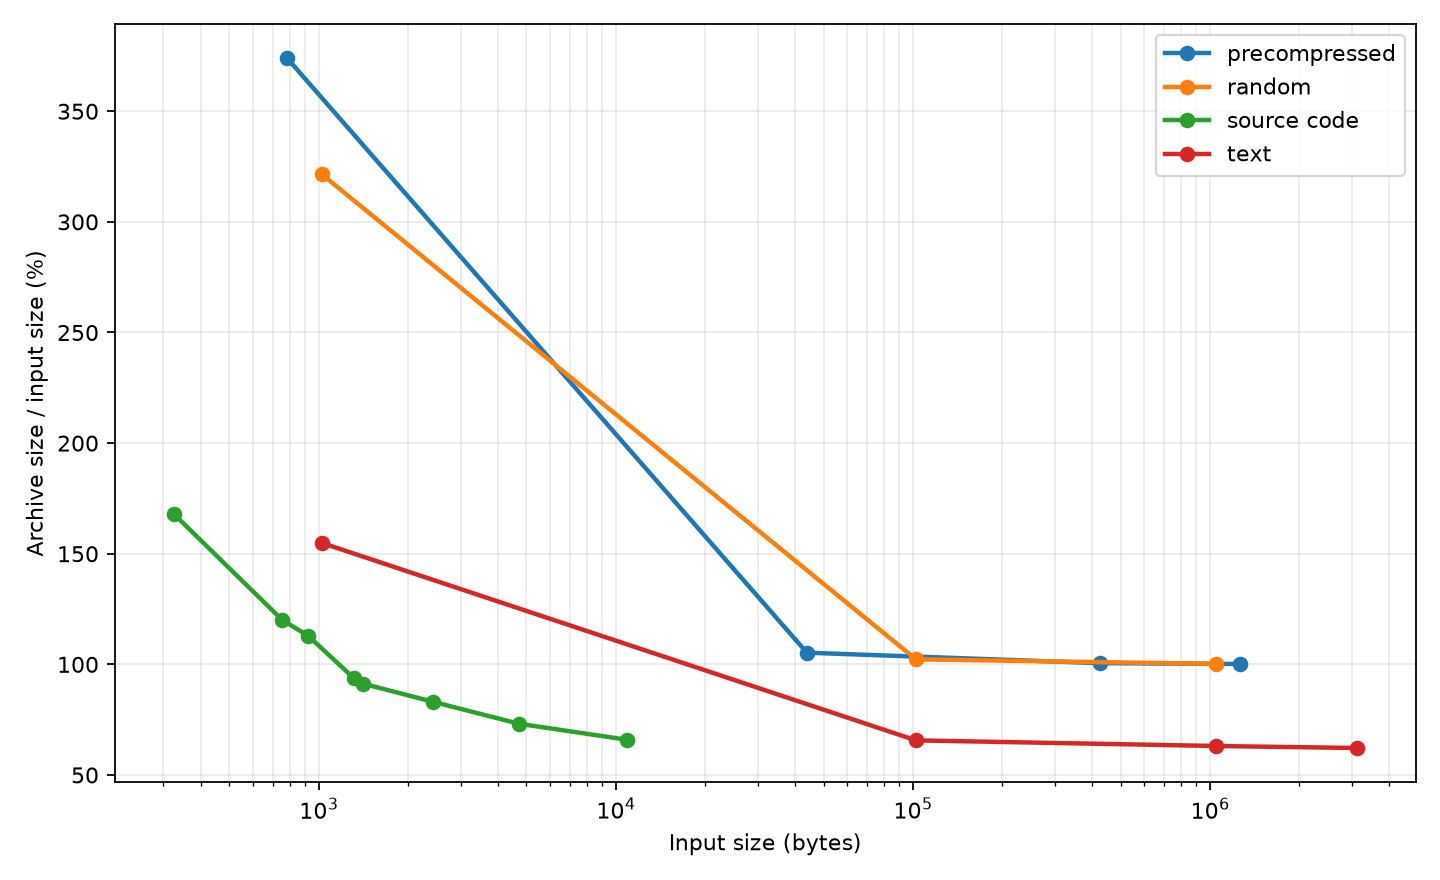
\includegraphics[width=\linewidth]{experiments/results/compression_ratio.png}
    \caption*{Размер архива относительно входа}
\end{minipage}\hfill
\begin{minipage}[t]{0.325\textwidth}
    \centering
    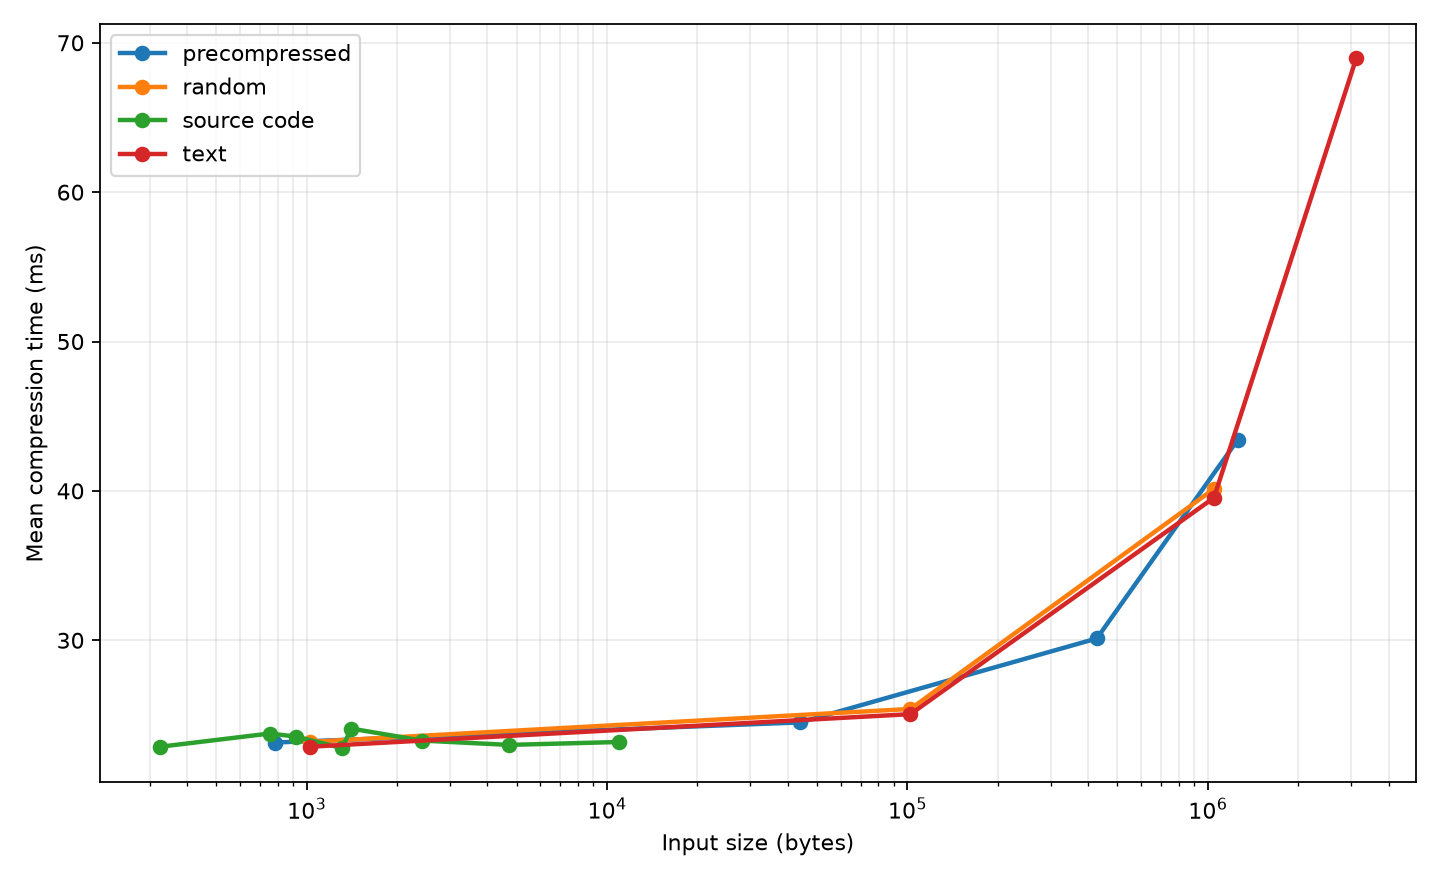
\includegraphics[width=\linewidth]{experiments/results/compression_time.png}
    \caption*{Время сжатия}
\end{minipage}\hfill
\begin{minipage}[t]{0.325\textwidth}
    \centering
    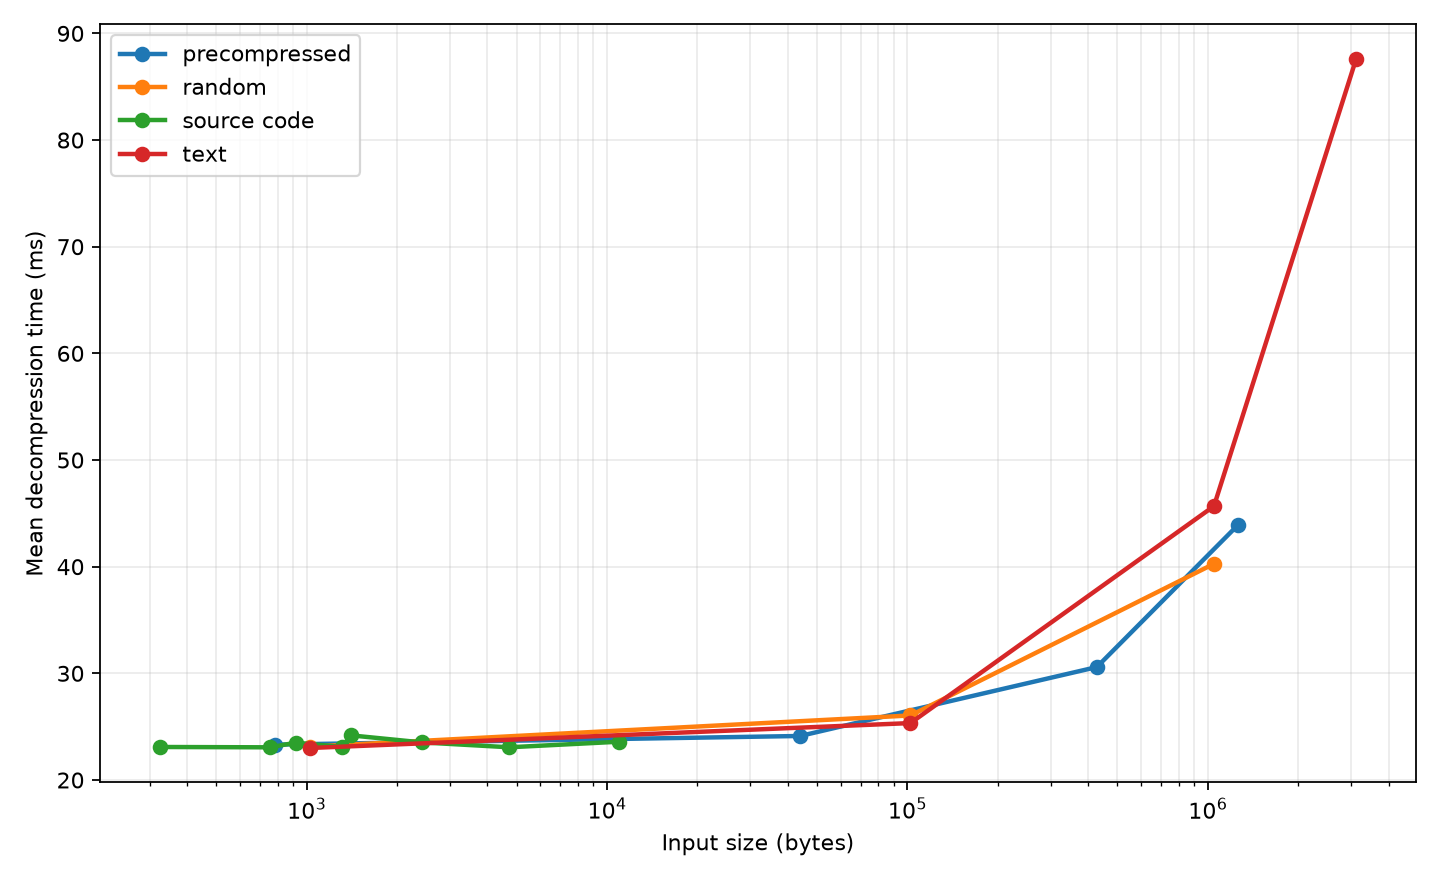
\includegraphics[width=\linewidth]{experiments/results/decompression_time.png}
    \caption*{Время распаковки}
\end{minipage}
\end{figure}

Для текстовых данных размер архива составил 62--66\% от исходного на файлах от 100 КиБ. На случайных данных размер архива близок к исходному для крупных файлов, но для файла 1 КиБ он достигает 321,5\% из-за заголовка и таблицы частот. Для ZIP-файлов превышение на крупных наборах составляет около 0,2\%. Результаты показывают, что эффективность зависит от структуры и размера входа.

\section{Заключение}
Разработан и проверен консольный архиватор без потерь с форматом HUF1. Реализованы построение кодов Хаффмана, упаковка битового потока, восстановление файлов и проверка целостности заголовка. Подготовлены модульные и CLI-интеграционные тесты, воспроизводимый сценарий эксперимента, CSV-таблицы и графики. Материалы эксперимента находятся в каталоге \texttt{experiments/results}; сценарий и инструкция запуска --- в репозитории проекта.

Репозиторий: \url{https://github.com/dem0phob1a/huffman_archiver_dem0phob1a}.\\
Техническая документация: файл \texttt{README.md} в репозитории.\\
Статус: реализация и экспериментальные материалы подготовлены к передаче преподавателю для получения отзыва; промышленное внедрение не заявляется.

\end{document}
